\chapter{Experiments, Results and Analysis}\label{ch:design-experiments}
\initial{C}hapter ~\ref{ch:research-methodology} documents the design of the hardware and algorithmic implementations of the system that was used.
Section~\ref{sec:op-params} shows some of the results obtained in a configuration step and determining the limitations of the unprocessed data.
To evaluate the performance of the designs, several Test suites were planned which exploited the No Line of Sight (NLOS) issue seen in previous sections.
To provide NLOS, rather than systematically occlude an anchor and tag, a person walked a fixed path (see Figure~\ref{fig:occlude}) at random speeds whilst the data was being recorded.
This was done as to emulate a more realistic environment that the system would be used in.

Two trajectories were outlined for tests while the tag was in motion.
Table~\ref{tb:trajs} shows the waypoints of each of the trajectories.
Trajectory one is a quadrilateral whilst trajectory two is a combination of straight-line segments.
In these tests, the tag was moved along the chosen trajectory whilst NLOS occurred randomly due to a person walking.

\begin{figure}[ht!]
    \centering
    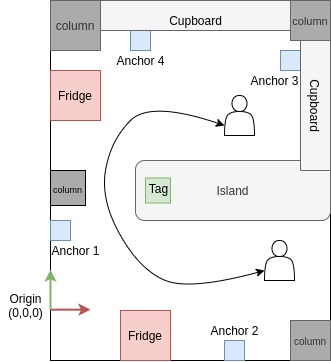
\includegraphics[scale=0.8]{Test_procedure}
    \caption{Path taken by the person to randomly occlude anchors and tag.}
    \label{fig:occlude}
\end{figure}

\begin{table}[ht!]
    \centering
    \begin{tabular}{|c|c|}
        \hline
        & Waypoints $(x,y)$(mm)\\
        \hline
        Trajectory 1 & $\begin{array}{c}
                            (1610, 2080)\\
                            (2111, 2080)\\
                            (1910, 2380)\\
                            (1610, 2580)\\
                            (1610, 2080)
        \end{array}$\\
        \hline
        Trajectory 2 & $\begin{array}{c}
                            (1610, 2080)\\
                            (1710, 2200)\\
                            (1760, 2300)\\
                            (1770, 2500)\\
                            (1840, 2580)\\
                            (1934, 2625)\\
                            (1992, 2595)
        \end{array}$\\
        \hline
    \end{tabular}
    \caption{Trajectories used in the tests for data collection.}
    \label{tb:trajs}
\end{table}
\newpage
\section{Design of Experiments}
\subsection{Benchmarking and Calibration}\label{sec:benchmarking}
Before testing the system with limitations a benchmark and calibration test was run to record results in an ideal scenario.
This test provided a base that can be used to compare the results of the system operating in non-ideal situations.
Figure ~\ref{fig:los} shows the results obtained for this benchmarking.
Although the measured position from the tag is slightly noisy, it is well within the $\pm10$cm accuracy quoted by the Pozyx system once the system has started moving and some time has passed.
\begin{figure}[h!]
    \centering
    \begin{subfigure}{0.6\textwidth}
            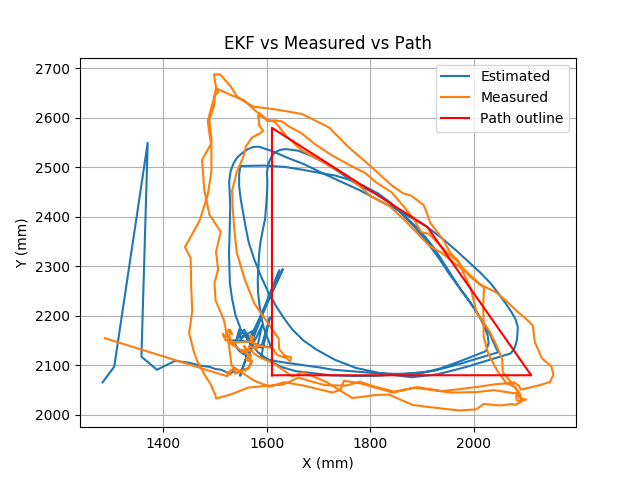
\includegraphics[width=\textwidth]{results/triangle_path_los}
            \caption{Person moving Tag on Trajectory 1.}
    \end{subfigure}
    \begin{subfigure}{0.6\textwidth}
            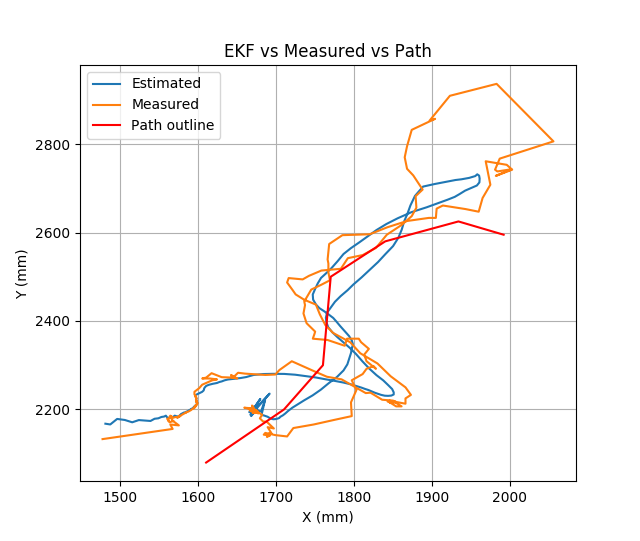
\includegraphics[width=\textwidth]{results/c_path_los}
            \caption{Person moving Tag on Trajectory 2.}
    \end{subfigure}
    \caption{Results for estimation with Line of Sight}
    \label{fig:los}
\end{figure}

\subsection{Stationary Tags}\label{sec:stationary-tags2}
For these evaluations the designed system was tested with stationary tags, similar to what was done in Section~\ref{sec:op-params}.
These were carried out to cover the trivial cases where NLOS proved to be an issue for even a stationary tag.
For the stationary tag tests, the tag was placed at a known point in the workspace and it was introduced to the basic limitations discussed previously.
The results for the loss of a single anchor was no different than the case recorded previously without the EKF .
However, Figure ~\ref{fig:stat_anchors} shows the results obtained with the tags located at various positions whilst a person walks randomly in the environment.
In contrast to the previous section, it can be seen that the system with the current configuration and EKF is able to withstand NLOS between the anchors and the tag with minimal change in the perceived position.
However, it is evident that the system is now susceptible to a steady-state error which is expected due to the Pozyx's integration with an IMU .
The tag's position will not change drastically and this error will be present as long as the tag is stationary.

\begin{figure}[h!]
    \centering
    \begin{subfigure}{0.49\textwidth}
            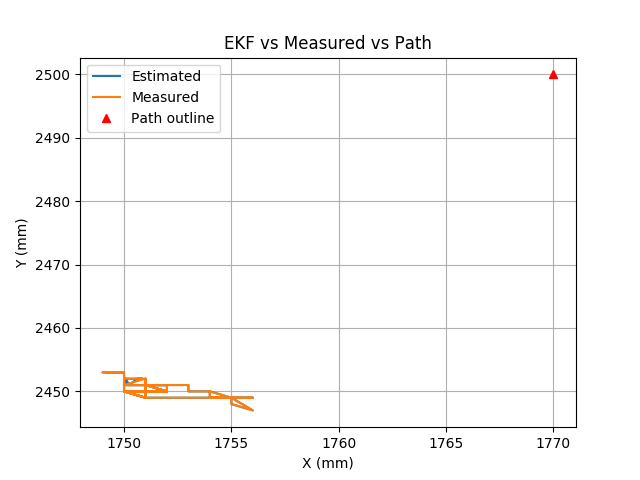
\includegraphics[width=\textwidth]{results/stationary_nlos_(1770,2500)}
            \caption{Result with tag at (1770,2500)}
    \end{subfigure}
    \begin{subfigure}{0.49\textwidth}
            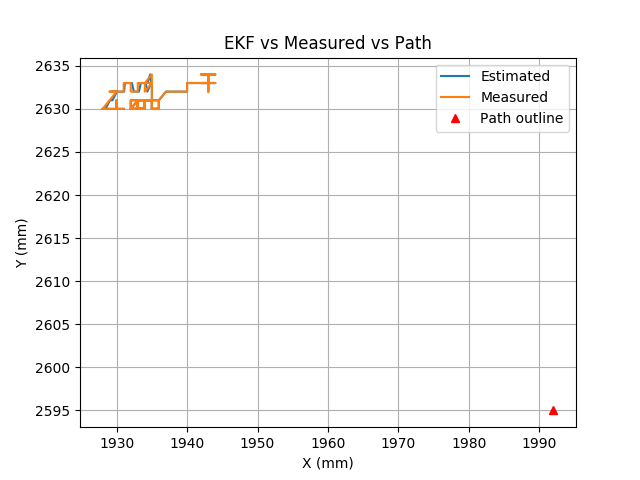
\includegraphics[width=\textwidth]{results/stationary_nlos_(1992,2595)}
            \caption{Result with tag at (1992,2595)}
    \end{subfigure}
    \begin{subfigure}{0.5\textwidth}
            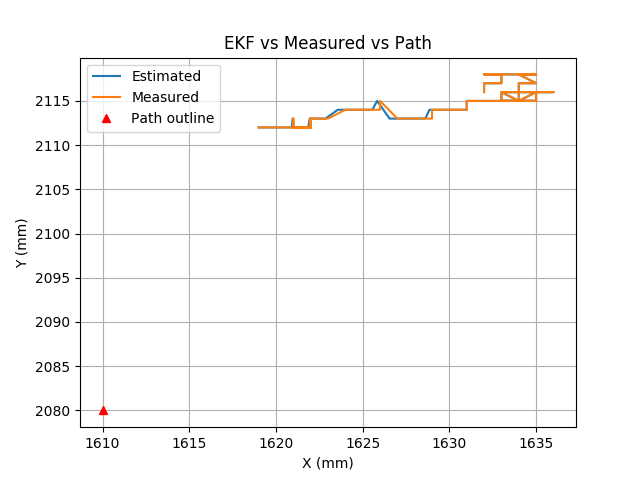
\includegraphics[width=\textwidth]{results/stationary_nlos_origin}
            \caption{Result with tag at (1610,2080)}
    \end{subfigure}
    \caption{Results obtained with No Line of Sight and a Stationary Tag.}
    \label{fig:stat_anchors}
\end{figure}
\newpage

\subsection{Localisation of a moving target}\label{sec:localisation-of-a-moving-target}
The following experiments would evaluate the designed system while the tag was moving.
This test was done to determine if the processing on the Pozyx tag in addition to an EKF would be able to provide suitable position estimates without the need for any additional measurements or processing.
Figure~\ref{fig:nlos_ppl} shows the paths recorded for each of these trajectories while the tag was moved by a single person.
It can be seen that as expected the EKF smoothens the supposed trajectory providing a better estimate.
Noteworthy is that using the IMU on the Pozyx tag causes the position to veer slightly on turns.
Additionally, the Pozyx tag was mounted onto a mobile robot that was built to follow a line.
This secondary setup was used to ensure that there was no interference from the person moving the tag and any errors seen would be due to the NLOS caused by the person walking in the environment as seen in Figure ~\ref{fig:occlude}.
Furthermore, using the mobile robot would indicate if the position estimates would be viable in a fully autonomous scenario.
Figure~\ref{fig:romi_nlos_1} shows the result obtained while the robot followed Trajectory 2 over two seperate runs.
\begin{figure}[ht!]
    \centering
    \begin{subfigure}{0.7\textwidth}
            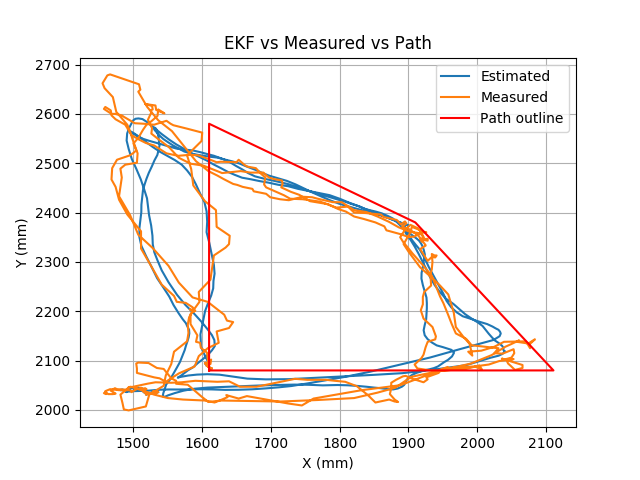
\includegraphics[width=\textwidth]{results/traingle_path_human(nlos)}
            \caption{Movement along Trajectory 1}
    \end{subfigure}
    \begin{subfigure}{0.7\textwidth}
            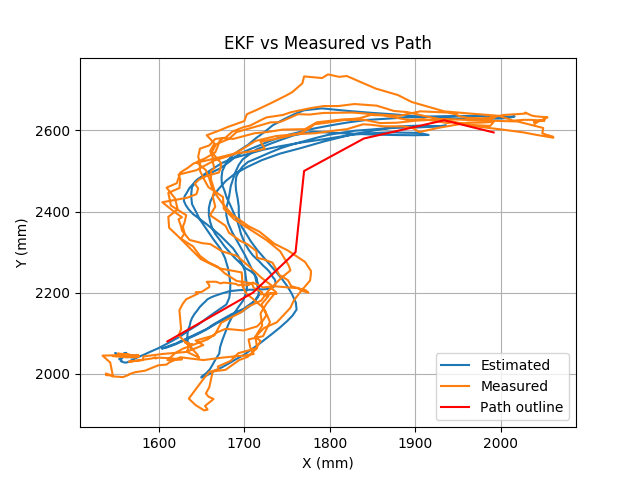
\includegraphics[width=\textwidth]{results/movement_along_c_path_human}
            \caption{Movement along Trajectory 2}
    \end{subfigure}
    \caption{Results obtained with No Line of Sight while the tag is moved by a person.}
    \label{fig:nlos_ppl}
\end{figure}

\begin{figure}[ht!]
    \centering
    \begin{subfigure}{0.7\textwidth}
            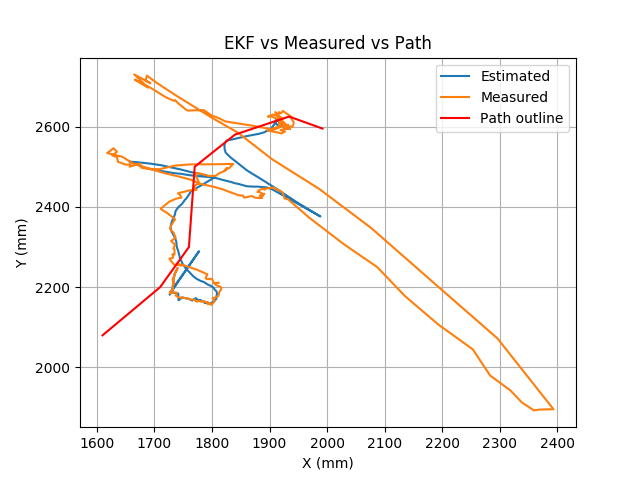
\includegraphics[width=\textwidth]{results/romi_c_path_2}
    \end{subfigure}
    \begin{subfigure}{0.7\textwidth}
            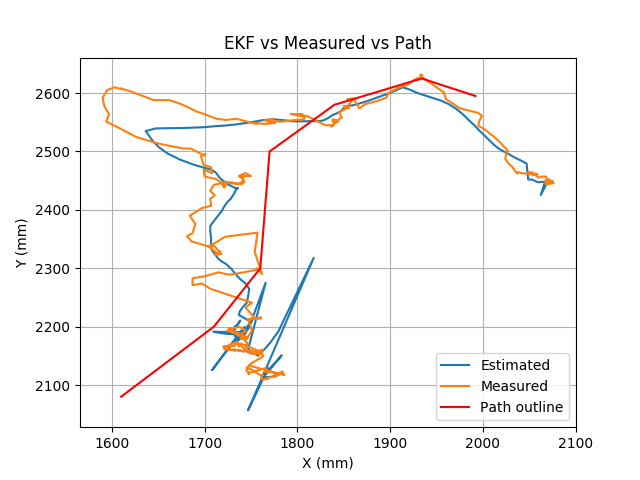
\includegraphics[width=\textwidth]{results/romi_ekf_c_path}
    \end{subfigure}
    \caption{Results obtained with No Line of Sight while the tag was mounted on the mobile robot.}
    \label{fig:romi_nlos_1}
\end{figure}

\subsection{Improving the Estimates}\label{sec:improving-the-estimates}
In UAVs there are different sensors that provide multiple measurements of the same state.
As discussed in Section~\ref{sec:sensor_fusion} it is useful to combine multiple sensor readings in order to improve the overall estimate of the state.
In Section~\ref{subsec:sensor-fusion} two methods of using the EKF was discussed.
For previous sections of this chapter, the input of the EKF consisted only of the measurements from the Pozyx tag.
In order to compliment the Pozyx measurements, dead reckoning data from the mobile robot was also used as an input into the EKF .
Figure ~\ref{fig:romi_los} shows the results obtained when the system was run in an ideal situation (Line of Sight).
This was done to once again set a base for comparing the No Line of Sight results.
Figure ~\ref{fig:romi_nlos_ekf} shows the results obtained from three separate runs of the robot.
The plots show, the actual path taken by the robot, the readings from the Pozyx tag, the readings from the dead reckoning system and the output of the EKF .
\begin{figure}[ht!]
    \centering
    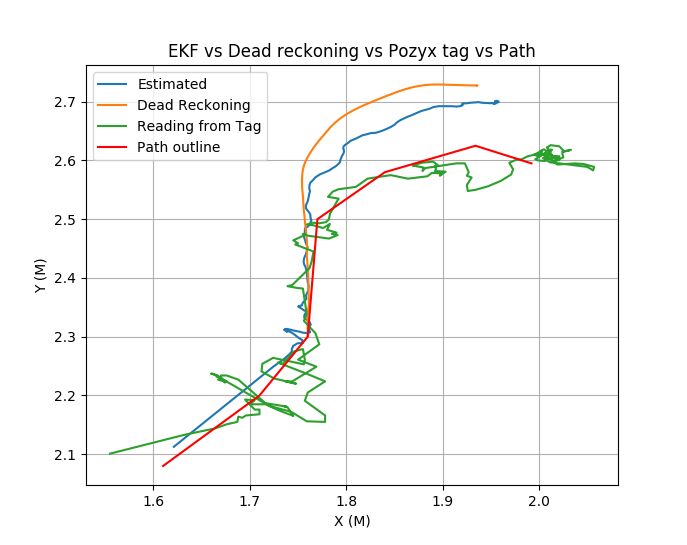
\includegraphics[scale=0.75]{results/romi_ekf_los}
    \caption{Line of Sight estimates from EKF using dead reckoning and Pozyx readings.}
    \label{fig:romi_los}
\end{figure}

\begin{figure}[ht!]
    \centering
    \begin{subfigure}{0.7\textwidth}
            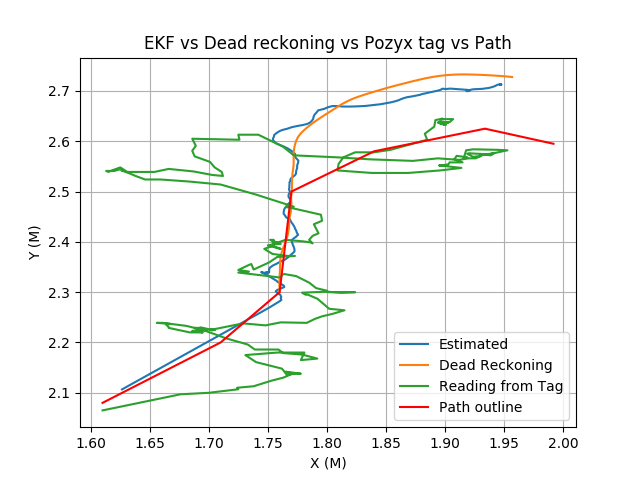
\includegraphics[width=\textwidth]{results/romi_ekf_less_good}
    \end{subfigure}
    \begin{subfigure}{0.7\textwidth}
            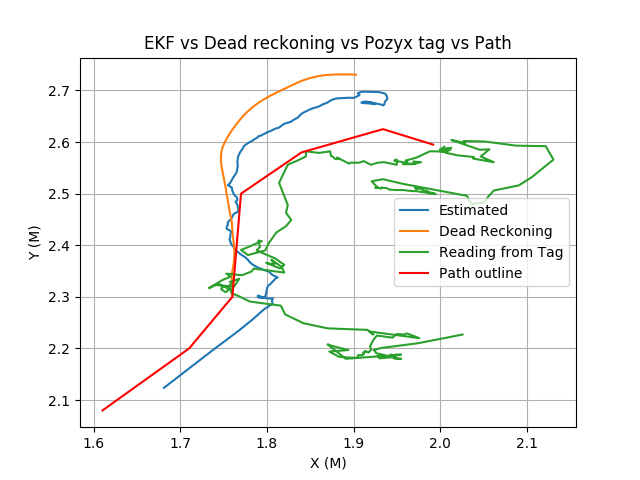
\includegraphics[width=\textwidth]{results/romi_ekf_embed_good_sink_start}
    \end{subfigure}
    \caption{Results obtained with No Line of Sight and EKF estimates using both dead reckoning and Pozyx readings.}
    \label{fig:romi_nlos_ekf}
\end{figure}
\begin{figure}[ht!]\ContinuedFloat
    \centering
    \begin{subfigure}{0.7\textwidth}
            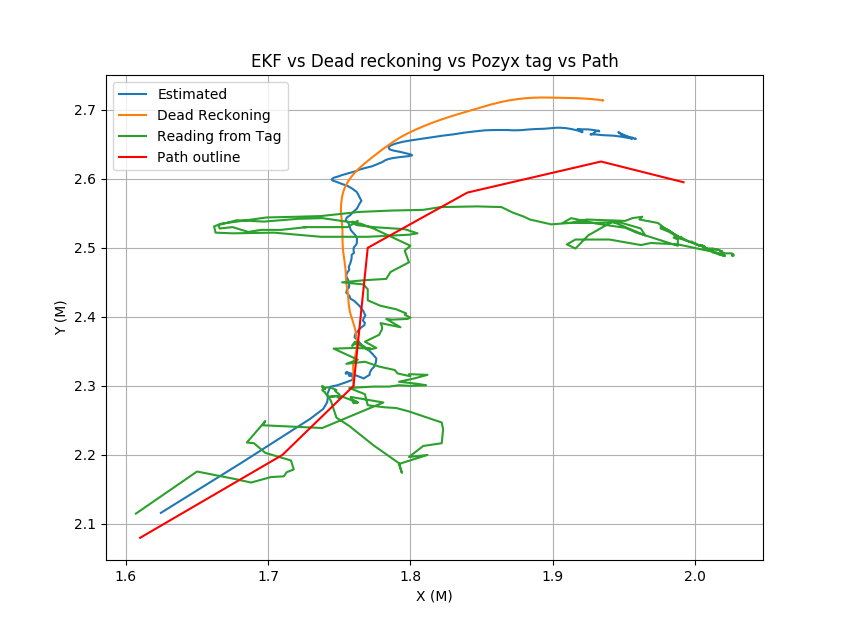
\includegraphics[width=\textwidth]{results/romi_ekf_embed_good}
    \end{subfigure}
    \caption[]{Results obtained with No Line of Sight and EKF estimates using both dead reckoning and Pozyx readings. (cont'd)}
\end{figure}
\newpage

\chapter{Results and Analysis}\label{ch:results-and-analysis}
\initial{T}o document the effectiveness of the Pozyx setup results were gathered in several scenarios.
Section: ~\ref{sec:op-params} shows some of the results obtained in a configuration step and determining the limitations of the unprocessed data.
In this chapter we will aim to show the effectiveness of the developed system and its feasibility in a kitchen which is known to have dynamic obstacles(people) that provide NLOS.
The following tests were carried out:
\begin{enumerate}
    \item Stationary tag with EKF and loss of a single anchor.
    \item Stationary tag with EKF and a person randomly moving in the environment providing random NLOS between various anchors and the tag.
    \item A person moving the anchor along 2 fixed paths with NLOS.
    \item A wheeled mobile robot programmed to follow a line using only the Pozyx tag measurements and EKF with NLOS.
    \item A wheeled mobile robot programmed to follow a line using dead reckoning, Pozyx measurements and an EKF with NLOS.
\end{enumerate}

%TODO: add in standard results and those DIST meatrics

Tests 1-2 were carried out to cover the trivial cases as seen in ~\ref{sec:op-params} where NLOS proved ot be an issue for even a stationary tag.
Test 3 was done to see if the processing on the Pozyx tag in addition to an EKF would be able to provide suitable pose estimates without the need for any additional measurements.
Test 4 provides a similar setup to Test 3 but with the added effect of the robot being able to accurately and consistently pass though desired waypoints.
Finally, Test 5 repeats the waypoint following of tests 3-4 but with the embedded EKF fusing both dead reckoning data and Pozyx tag readings.
To provide NLOS, rather than systematically occlude an anchor and tag, a person walked a fixed path (see Figure:~\ref{fig:occlude}) at random speeds whilst the data was being recorded.
This was done as to emulate a more realistic environment that the system would be used in.

\begin{figure}[ht!]
    \centering
    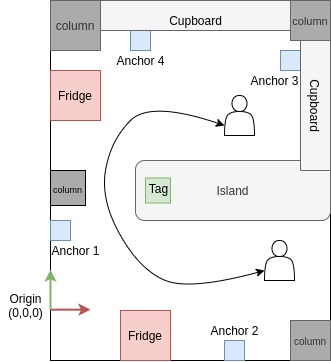
\includegraphics[scale=0.8]{Test_procedure}
    \caption{Path taken by the person to randomly occlude anchors and tag.}
    \label{fig:occlude}
\end{figure}
To set a benchmark, the tests while the Pozyx tag was in motion was run initially with ideal line of sight between the anchors and the tag.
Figure: ~\ref{fig:los} shows the results obtained for this benchmarking.
It is seen although the measured position from the tag is slightly noisy, it is well within the $\pm10$cm accuracy quoted by the Pozyx system once the system has started moving and some time has passed.
Table:~\ref{tb:results} shows some statistics gathered from these ideal scenario tests highlighted in blue and will be discussed later on.

\begin{figure}[h!]
    \centering
    \begin{subfigure}{0.49\textwidth}
            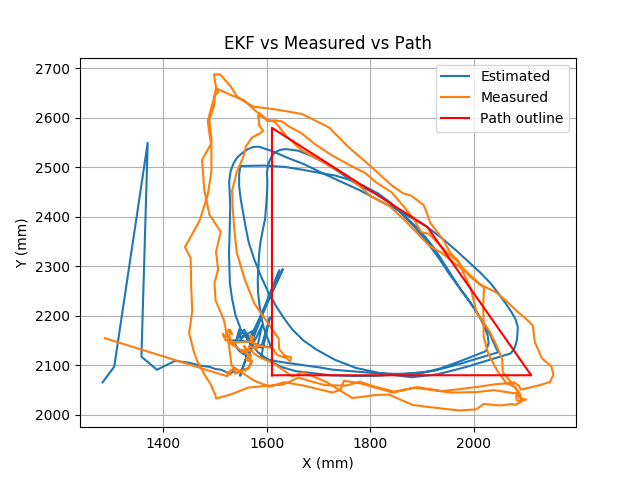
\includegraphics[width=\textwidth]{results/triangle_path_los}
            \caption{Person moving Tag on Trajectory 1.}
    \end{subfigure}
    \begin{subfigure}{0.49\textwidth}
            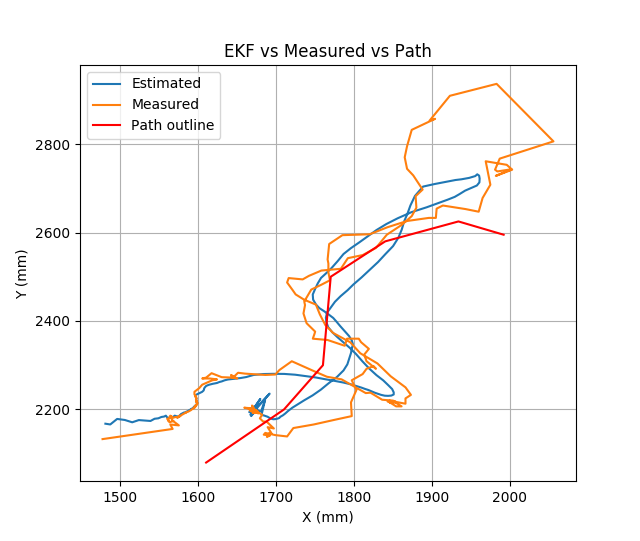
\includegraphics[width=\textwidth]{results/c_path_los}
            \caption{Person moving Tag on Trajectory 2.}
    \end{subfigure}
    \begin{subfigure}{0.5\textwidth}
            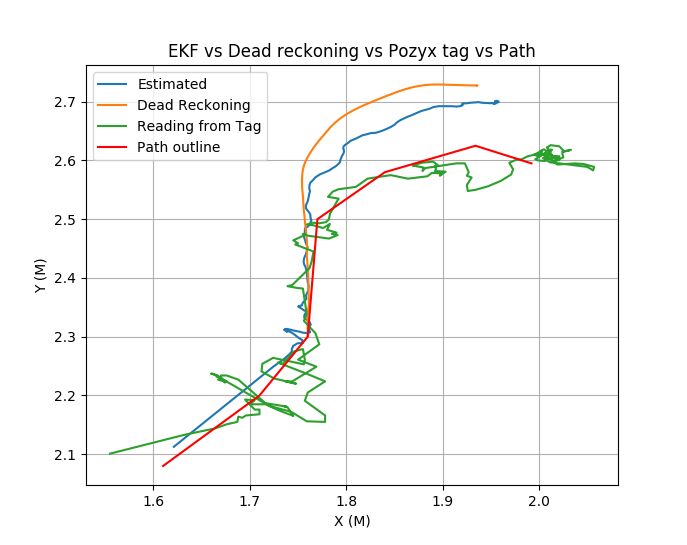
\includegraphics[width=\textwidth]{results/romi_ekf_los}
            \caption{WMR equipped with Tag on Tajectory 2.}
    \end{subfigure}
    \caption{Results for estimation with Line of Sight}
    \label{fig:los}
\end{figure}
\newpage
\section{Stationary Tags}\label{sec:stationary-tags}
For the stationary tag tests, the tag was placed at a known point in the workspace and it was introduced to the basic limitations discussed in previous chapters.
The results for the loss of a single anchor was no different than the case recorded previously without the EKF .
However, Figure: ~\ref{fig:stat_anchors} shows the results obtained with the tags located at various positions whilst a person walks randomly in the environment.
In contrast to the previous section, it can be seen the system with the current configuration and EKF is able to withstand NLOS between the anchors and the tag with minimal change in the perceived position.
However, it is evident that the system is now susceptible to a steady-state error which is expected due to the Pozyx's integration with an IMU .
The tag's position will not change drastically and this error will be present as long as the tag is stationary.
The following sections will have the Pozyx time in motion so this error is expected to reduce.

\begin{figure}[h!]
    \centering
    \begin{subfigure}{0.49\textwidth}
            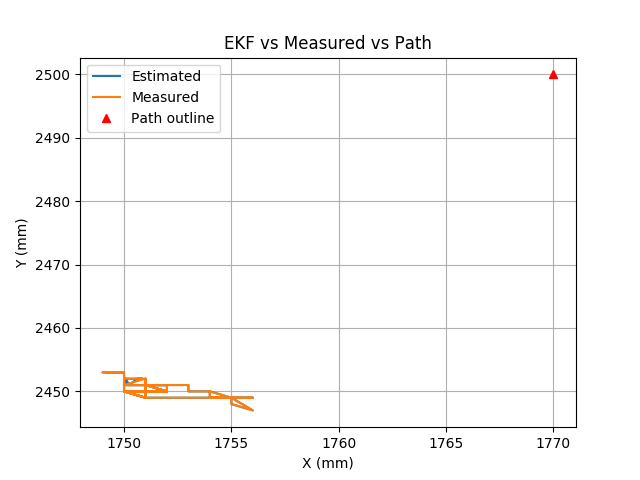
\includegraphics[width=\textwidth]{results/stationary_nlos_(1770,2500)}
            \caption{Result with tag at (1770,2500)}
    \end{subfigure}
    \begin{subfigure}{0.49\textwidth}
            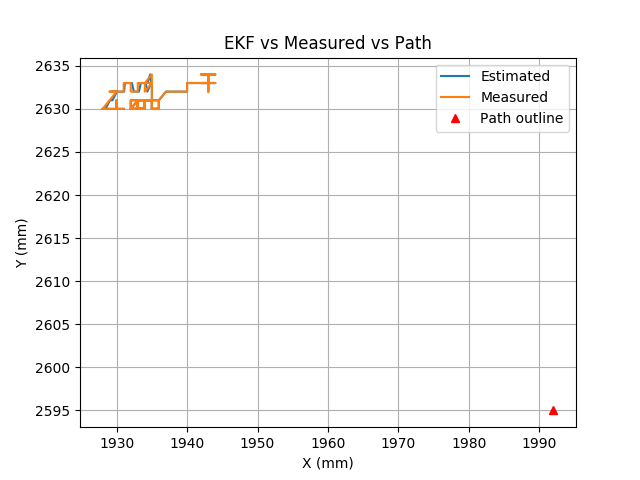
\includegraphics[width=\textwidth]{results/stationary_nlos_(1992,2595)}
            \caption{Result with tag at (1992,2595)}
    \end{subfigure}
    \begin{subfigure}{0.5\textwidth}
            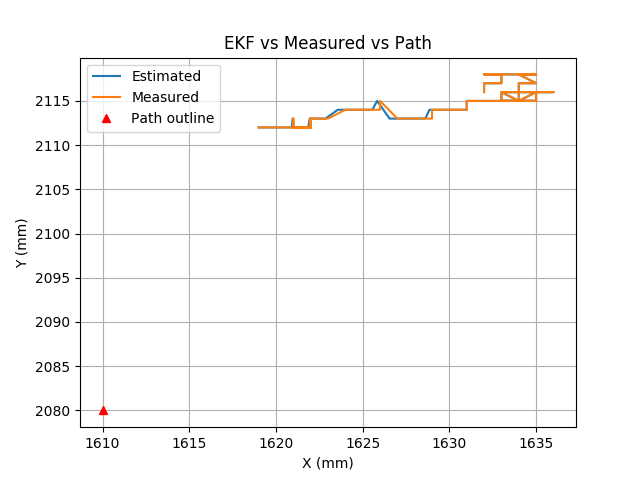
\includegraphics[width=\textwidth]{results/stationary_nlos_origin}
            \caption{Result with tag at (1610,2080)}
    \end{subfigure}
    \caption{Results obtained with NLOS and a single anchor.}
    \label{fig:stat_anchors}
\end{figure}
\newpage
\section{Person moving the tag}\label{sec:person-moving-the-tag}
Two trajectories were outlined for these subsets of tests.
Table:~\ref{tb:trajs} shows the waypoints of each of the trajectories.
Trajectory one is a quadrilateral whilst trajectory two is a combination of straight-line segments.
In these tests, the tag was moved along the chosen trajectory whilst NLOS occurred randomly due to a person walking.
\begin{table}[ht!]
    \centering
    \begin{tabular}{|c|c|}
        \hline
        & Waypoints $(x,y)$(mm)\\
        \hline
        Trajectory 1 & $\begin{array}{c}
                            (1610, 2080)\\
                            (2111, 2080)\\
                            (1910, 2380)\\
                            (1610, 2580)\\
                            (1610, 2080)
        \end{array}$\\
        \hline
        Trajectory 2 & $\begin{array}{c}
                            (1610, 2080)\\
                            (1710, 2200)\\
                            (1760, 2300)\\
                            (1770, 2500)\\
                            (1840, 2580)\\
                            (1934, 2625)\\
                            (1992, 2595)
        \end{array}$\\
        \hline
    \end{tabular}
    \caption{Trajectories used in the tests for data collection.}
    \label{tb:trajs}
\end{table}
Figure:~\ref{fig:nlos_ppl} shows the paths recorded for each of these trajectories.
It can be seen that as expected the EKF smoothens the supposed trajectory providing a better estimate.
Noteworthy is that using the IMU on the Pozyx tag causes the position to veer slightly on turns.
\begin{figure}[ht!]
    \centering
    \begin{subfigure}{0.7\textwidth}
            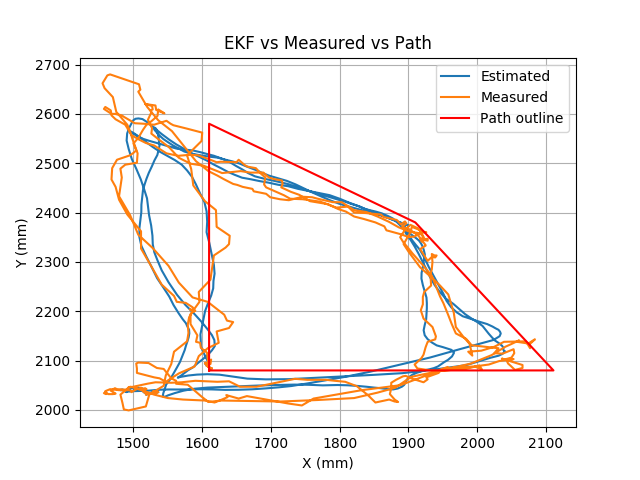
\includegraphics[width=\textwidth]{results/traingle_path_human(nlos)}
            \caption{Movement along Trajectory 1}
    \end{subfigure}
    \begin{subfigure}{0.7\textwidth}
            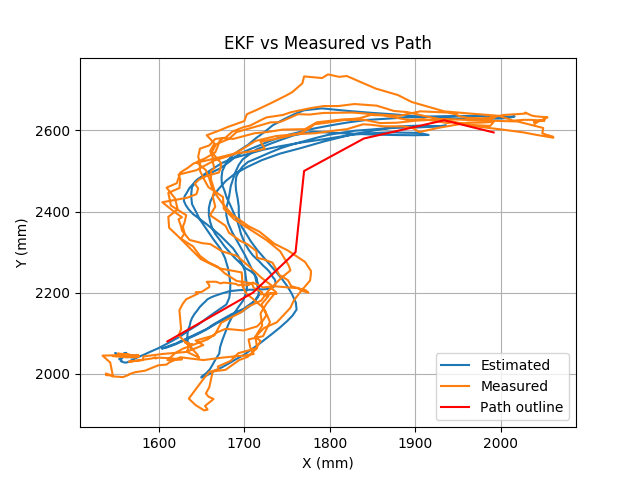
\includegraphics[width=\textwidth]{results/movement_along_c_path_human}
            \caption{Movement along Trajectory 2}
    \end{subfigure}
    \caption{Results obtained with NLOS while the tag is moved by a person.}
    \label{fig:nlos_ppl}
\end{figure}
\newpage
\section{Mobile robot results}\label{sec:mobile-robot-results}
For the final bit of tests, a wheels mobile robot was used.
The system is a simple differential drive robot equipped with wheel encoders to provide dead reckoning position estimates.
The data was collected in two modes:
\begin{enumerate}
    \item The tag was placed on the robot and the filter was used with the tag readings alone while the robot followed trajectory 2 above.
    \item The tag was integrated into the embedded system of the robot and the tag's reading was fused with the dead reckoning data whilst following trajectory 2.
\end{enumerate}
The primary driving force for these tests was to eliminate the person required to move the tag and see if the position estimates would be viable in an autonomous robotic scenario such as the case of a UAV using the Ardupilot firmware.
Figure:~\ref{fig:romi_nlos_1} shows the paths obtained for the test using the tag and EKF alone.
A major problem that arose with the measured values occurred when a turn was being made and NLOS.
Some of the measured points wildly deviated from the actual position of the robot, although the implemented EKF algorithm is able to reduce some of the noise it is still susceptible to these errors since it is the only measurement being used.
\begin{figure}[ht!]
    \centering
    \begin{subfigure}{0.7\textwidth}
            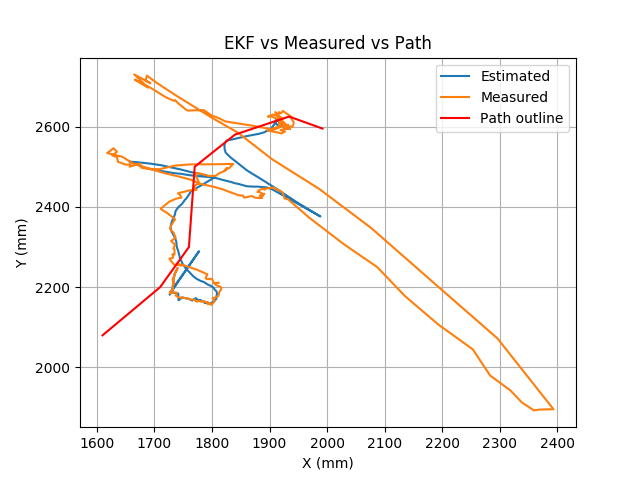
\includegraphics[width=\textwidth]{results/romi_c_path_2}
    \end{subfigure}
    \begin{subfigure}{0.7\textwidth}
            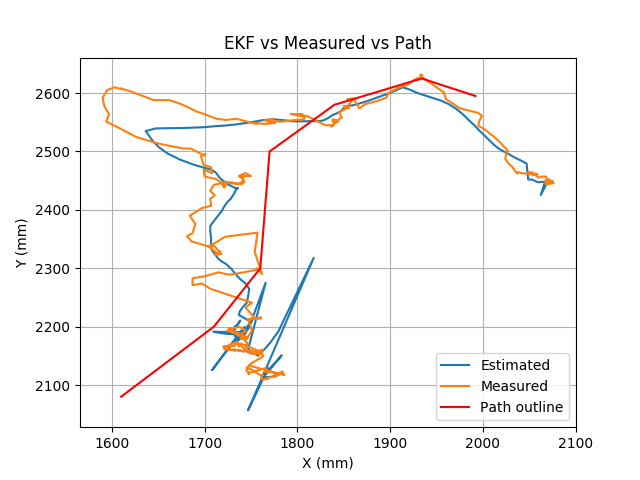
\includegraphics[width=\textwidth]{results/romi_ekf_c_path}
    \end{subfigure}
    \caption{Results obtained with NLOS while following Trajectory 2 on the WMR.}
    \label{fig:romi_nlos_1}
\end{figure}

\begin{figure}[ht!]
    \centering
    \begin{subfigure}{0.6\textwidth}
            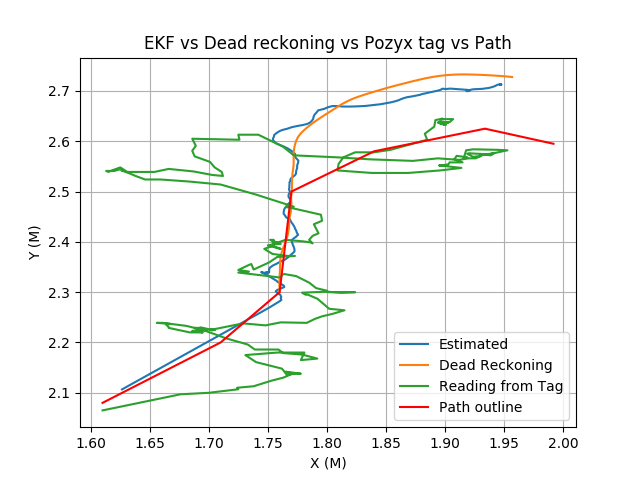
\includegraphics[width=\textwidth]{results/romi_ekf_less_good}
    \end{subfigure}
    \begin{subfigure}{0.6\textwidth}
            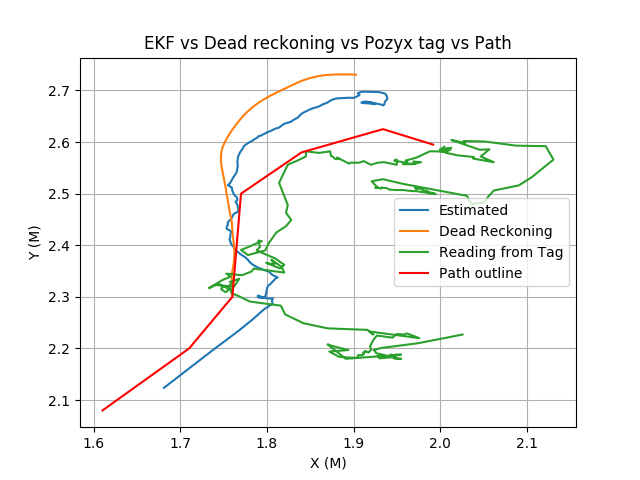
\includegraphics[width=\textwidth]{results/romi_ekf_embed_good_sink_start}
    \end{subfigure}
    \begin{subfigure}{0.6\textwidth}
            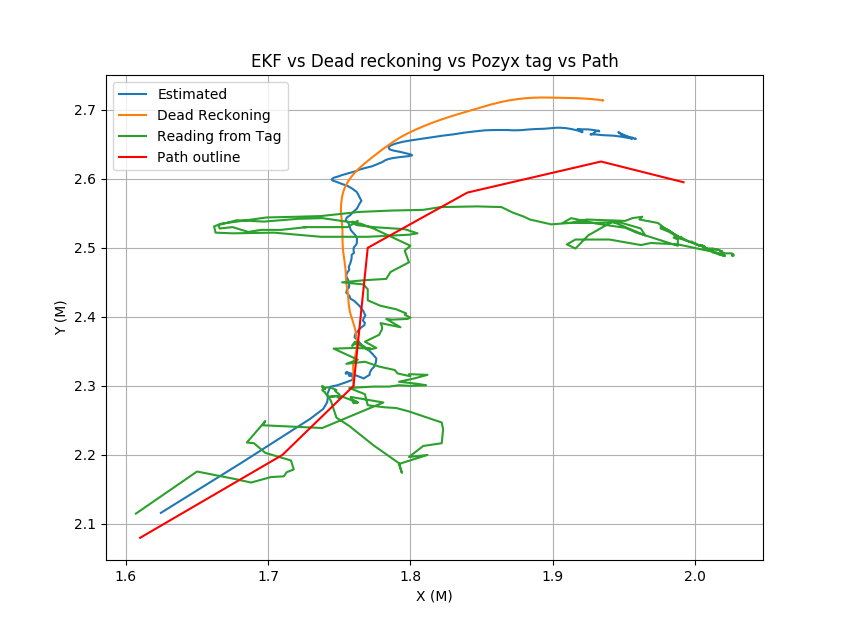
\includegraphics[width=\textwidth]{results/romi_ekf_embed_good}
    \end{subfigure}
    \caption{Results obtained with NLOS while following Trajectory 2 on the WMR with the embedded EKF.}
    \label{fig:romi_nlos_ekf}
\end{figure}
%\lipsum[2-10]
For the second test using the mobile robot, an embedded EKF was implemented.
Figure:~\ref{fig:romi_nlos_ekf} shows the result obtained from the fusion of the dead reckoning data and the Pozyx readings.
From the plots, it is clear that this implementation provides the best result when compared with the results gathered for Figures: ~\ref{fig:romi_nlos_1}, ~\ref{fig:nlos_ppl}.


\section{Analysis of Results}\label{sec:analysis-of-results}
From a qualitative point, the embedded EKF fusing the dead reckoning data and tag data seems to outperform the other methods in terms of falling close to the actual path and being robust to the erratic behaviour introduced by NLOS.
However, a useful metric would be to see the distance from the supposed positions to the path being traveled.
Since the robot moved autonomously and there was no perception of where it should be at a given time a way of effectively measuring the distance to the path needed to be designed.
Figure:~\ref{fig:dist} shows what is available while data is being recorded.
The green arrows represent the minimum distance for a candidate point and the path.
Appendix:~\ref{app:app04} shows the general pseudo-code to obtain the green distance for each point.
A benefit of using a distance metric is that it is easy to interpret and ideally should be zero if the pose estimates are completely accurate.
This also means that standard statistics on this distance metric would give a clear indication of which method produced the best results.
\begin{figure}[ht!]
    \centering
    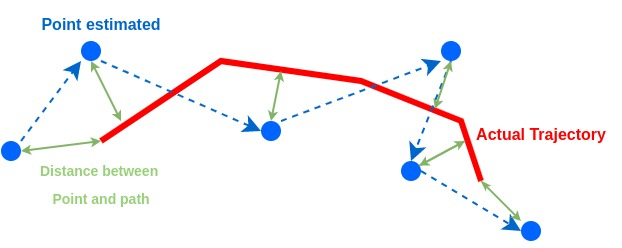
\includegraphics[scale=0.8]{dist_metrics}
    \caption{Illustration of how a distance metric was developed for analysis.}
    \label{fig:dist}
\end{figure}

\begin{table}[ht!]
    \centering
    \begin{tabular}{|c|c|c|c|c|c|}
        \hline
        & Max & Mean & Variance & Skew & Kurtosis \\
        \hline
        \rowcolor{LightNavy}Trajectory 1 by human (Tag) with LOS & 0.4031 & 0.115 & 0.007 & 1.219& 0.5642\\
        \hline
        \rowcolor{LightNavy}Trajectory 2 by human (Tag) with LOS & 0.1563 & 0.06 & 0.0016 &0.1164 & -1.432\\
        \hline
        \rowcolor{LightNavy}Trajectory 2 by WMR with LOS & 0.0795 & 0.04 & 0.0009 & -0.0735 & -1.7372\\
        \hline
        Trajectory 1 by human (Tag) & 0.331 & 0.114 & 0.006 & 0.7851 & -0.1624\\
        \hline
        Trajectory 2 by human (Tag) & 0.137 & 0.0431& 0.0009 & 1.0405 & 0.3421\\
        \hline
        Trajectory 2 by WMR (Tag) &  0.3297 & 0.05416 & 0.00189 & 1.0415 & 3.8087\\
        \hline
        \rowcolor{LightGreen}Trajectory 2 by WMR (Tag + Dead Reckoning)& 0.087 & 0.036 & 0.00047 & 0.1634 & -0.2665\\
        \hline
        Trajectory 2 by WMR(Dead Reckoning)& 0.1081 & 0.067 & 0.00136 & -0.9802 & -0.8165\\
        \hline
        Trajectory 2 by WMR (Tag) & 0.1124 & 0.069 & 0.00153 & -0.5188 & -1.352\\
        \hline
    \end{tabular}
    \caption{Metrics for the Distance from each path for different tests and positions.}
    \label{tb:results}
\end{table}

Table:~\ref{tb:results} shows the final metrics obtained for the various results.
In addition to the EKF fused results, the statistics for the tag and dead reckoning positions were included to set a benchmark for comparison.
As expected the estimates combining the dead reckoning and tag readings clearly outperforms the others.
The EKF implemented on the WMR is quite simple so it is expected that similar or even better results would be obtained on the FCU whilst in flight.

\section{Summary}
This chapter documented the experiments designed and ran in order to evaluate the performance of the Pozyx system for indoor localisation.
These tests were necessary as they addressed the feasibility of using the Pozyx system in UAVs and other forms of autonomous systems.
%In the next chapter the results will be discussed providing a qualitative and quantitative analysis of the plots seen in this section.
From the analysis of the results it is clear that the raw readings from the Pozyx system is prone to errors when NLOS is introduced but integrating a simple EKF is able to mitigate the errors a bit.
